\documentclass[a4paper,1pt]{report}
\usepackage[utf8]{inputenc}
\usepackage[spanish]{babel}
\usepackage{amsfonts}
\usepackage{amsthm}
\usepackage{amssymb}
\usepackage{amsmath}
\usepackage{graphicx}
\usepackage{subcaption}
\usepackage{float}
\usepackage[rightcaption]{sidecap}

\newtheorem*{pbo}{Principio del Buen Ordenamiento}

\newtheorem*{pim}{Principio de Inducción Matemática}

\newtheorem*{teo}{Teorema}

\newtheorem*{cor}{Corolario}

\newtheorem*{dem}{Demostración}

\newtheorem*{dfn}{Definición}

\newtheorem*{lem}{Lema}

\newtheorem*{prp}{Propiedades}


% Title Page
\title{Conferencia 7 - Emparejamiento}
\author{}

\begin{document}
\maketitle

\begin{dfn}
 Sea $G=<V,E>$ un grafo, dos aristas de G son independientes sin no tienen un vértice en común.
\end{dfn}


\begin{dfn}
    Un emparejamiento~(\textit{matching}) en G es un conjuntos de aristas independientes dos a dos.
\end{dfn}

\begin{figure}[H]
    \centering
    \begin{subfigure}[b]{0.40\textwidth}
        \centering
        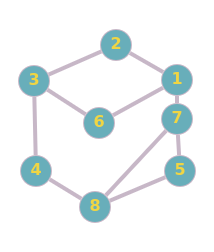
\includegraphics[width=0.4\textwidth]{figures7/grafo.png}
        \caption{Grafo $G$}
    \end{subfigure} 
    \begin{subfigure}[b]{0.40\textwidth}
        \centering
        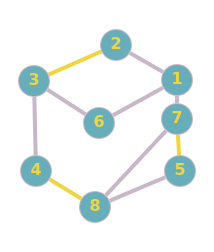
\includegraphics[width=0.4\textwidth]{figures7/matching.png}
        \caption{Emparejamiento en $G$}
    \end{subfigure}
    \caption{En la figura las aristas $\{ 4,8\}, \{2,3\}$ y $\{7,5\}$ son independientes dos a dos, por lo que forman un emparejamiento}
\end{figure} 

\begin{dfn}
 Un emparejamiento M se dice que satura a un vértice v de G si v es un extremo de una arista en M.
\end{dfn}

\begin{dfn}
 Se dice que M satura a $X\subseteq V(G)$ si satura a todo v tal que $v\in X$
\end{dfn}

\begin{figure}[H]
        \centering
        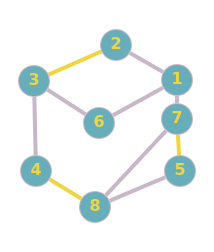
\includegraphics[width=0.2\textwidth]{figures7/matching.png}
        \caption{En la figura el emparejamiento satura a $X = \{2,3,4,5,7,8\}$}
    \end{figure} 
    
    \begin{dfn}
        Si M satura a V(G) entonces se dice que M es un emparejamiento perfecto.
    \end{dfn}
    
    \begin{figure}[H]
        \centering
        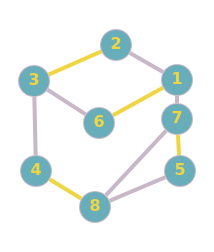
\includegraphics[width=0.2\textwidth]{figures7/maximo.png}
        \caption{En la figura el emparejamiento satura a $V(G)$ por lo que es perfecto}
\end{figure} 


\begin{dfn}
 Un emparejamiento es maximal si no se puede adicionar ninguna arista a M que sea independiente con todas las pertenecientes a M.
\end{dfn}

\begin{figure}[H]
    \centering
    \begin{subfigure}[b]{0.40\textwidth}
        \centering
        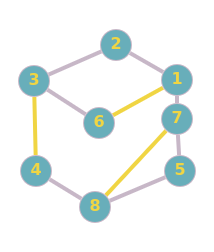
\includegraphics[width=0.4\textwidth]{figures7/maximal.png}
    \end{subfigure} 
    \begin{subfigure}[b]{0.40\textwidth}
        \centering
        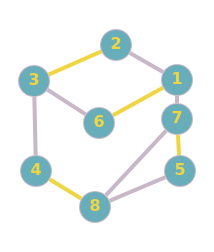
\includegraphics[width=0.4\textwidth]{figures7/maximo.png}
    \end{subfigure}
    \caption{Los emparejamientos formados en ambos ejemplos al tomar las aristas resaltadas, son maximales, agregar cualquier otra arista viola la definici\'on de emparejamiento}
\end{figure} 

\begin{dfn}
 Un emparejamiento es máximo si tiene la mayor cardinalidad entre todos los emparejamientos
\end{dfn}


\begin{dfn}
 Sea G un grafo y M un emparejamiento de G:
 \begin{itemize}
  \item Un camino M-alternativo es un camino simple cuyas aristas alternan entre aristas que están en M y aristas que no están en M
  \item Si el camino M-alternativo comienza y termina en vértices no saturados por M se dice que es un camino M-incremento
 \end{itemize}
\end{dfn}

\begin{figure}[H]
    \centering
    \begin{subfigure}[b]{0.80\textwidth}
        \centering
        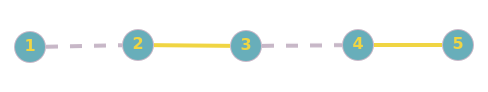
\includegraphics[width=0.7\textwidth]{figures7/malternativo.png}
        \caption{Camino M-alternativo}
    \end{subfigure} 
    \begin{subfigure}[b]{0.70\textwidth}
        \centering
        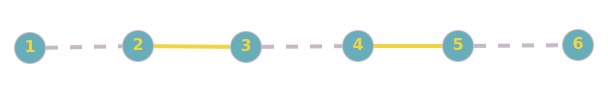
\includegraphics[width=0.9\textwidth]{figures7/mincremento.png}
        \caption{Camino M-incremento}
    \end{subfigure}
\end{figure} 

\begin{lem}
 En un grafo G conexo tal que para todo vértice  v de G se tiene que el grado de v es menor o igual a 2 entonces G es un camino simple o un ciclo.
\end{lem}

\begin{dem}
 
\end{dem}

Si $|V(G)| = 1$ es trivial.

Para demostrar que $G$ con $|V(G)| >1$ es $P_n$ o $C_n$, tomemos el camino simple maximal $c=<v_1,v_2,\dots,v_{k-1},v_k>$ (que sabemos existe puesto que en G hay a menos una arista ya que todo grafo conexo con $|V(G)| > 1$ los v\'ertices tienen grado mayor o igual a 1)

Es necesario demostrar que toda arista de $G$ pertenece a $c$ salvo quizas la arista $\{v_1,v_k\}$. Para ellos analicemos para cada v\'ertice de $c$ las aristas que inciden en ellos.

\begin{itemize}
    \item[] Para $v_i, \ 1<i< k$, es decir para los v\'ertices intermedios del camino, como todos los v\'ertices de $G$ tienen grado menor o igual a 2, y para cada uno en $c$ est\'an las aristas $\{v_{i-1}, v_i\}$ y $\{v_i, v_{i+1}\}$, toda arista que incide en $v_i$ est\'a en el camino.
    \item[] Para $v_1$ y $v_k$, o sea, los v\'ertices extremos del camino, sabemos que est\'an conectados a $c$ por las aristas $\{v_1, v_2\}$ y $\{v_{k-1}, v_k\}$ respectivamente, de donde para ambos se cumple que solo es posible tener un adyacente m\'as, pero para ning\'un otro v\'ertice intermedio puede existir una conexi\'on con $v_1$ o $v_k$, puesto que en el caso que analizamos anteriormente se evidencia que los vertices intermedios solo est\'an conectados a su antecesor y a su sucesor en el camino y no pueden tener m\'as adyacentes porque su grado m\'aximo es 2. Adem\'as no puede ser que $v_1$ o $v_k$ sean adyavcentes a un $w \notin c$ porque que $c$ es m\'aximo. De modo que solo es posible para $v_1$ y $v_k$ que exista la arista $\{v_1, v_k\}$.
\end{itemize}

En caso que $\{v1, v_k\} \in G$, $G$ ser\'ia $C_n$ y en caso contrario $P_n$ $\blacksquare$.


\begin{teo}
 Sea $G=<V,E>$ un grafo, un emparejamiento M de G es máximo si y solo si no existen en G caminos M-incremento
\end{teo}


\begin{dem}
La demostración es equivalente a demostrar que M no es máximo si y solo si existe algún camino M-incremento en G. 
\end{dem}

\begin{dem}[$\Rightarrow$]
    Si existe algún camino M-incremento entonces M no es máximo
\end{dem}

Si existe algún camino M-incremento este será de la forma:

\textit{no-si-no-si-...-no-si-no}

\begin{figure}[H]
    \centering
    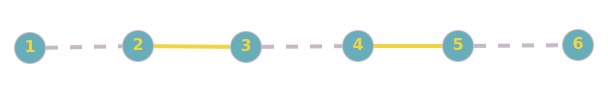
\includegraphics[width=0.6\textwidth]{figures7/mincremento.png}
\end{figure} 

Las aristas \textit{no} de este camino distintas a las de los extremos contienen vértices que están saturados por el emparejamiento.

Si en el emparejamiento se sustituyen las aristas \textit{si} por las \textit{no}, se obtiene uno nuevo que tiene mayor tamaño, puesto que las aristas \textit{no}  exceden en 1 a las \textit{si}.
\begin{figure}[H]
    \centering
    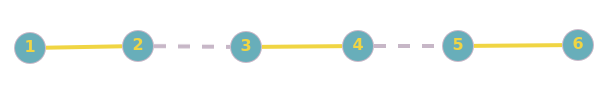
\includegraphics[width=0.6\textwidth]{figures7/mnoincremento.png}
\end{figure} 

Esto se puede realizar sin problemas pues ningún otro vértice saturado del emparejamiento anterior está en el camino, lo que implica que las aristas que no aparecían en él no se ven comprometidas.\\

\begin{dem}[$\Leftarrow$]
    Si M no es máximo entonces existe algún camino M-incremento
\end{dem}

Como $M$ no es m\'aximo, entonces $\exists M'$ tal que $|M'| > |M|$.\\

Sea la operación diferencia simétrica:

$A\bigtriangleup B = (A/B) \cup (B/A) = (A\cup B) / (A\cap B)$

Entonces, volvamos a la demostración:

Tomemos el conjunto $M'\bigtriangleup M$ en el cual hay al menos una arista pues \\
$|M'|>|M|$. Entonces tomemos todas las componentes conexas de $M'\bigtriangleup M$ que contienen aristas. 

Note que todos los vértices de $M'\bigtriangleup M$ tienen grado menor o igual a 2, puesto que para cada v\'ertice puede ocurrir uno de estos casos:
\begin{itemize}
 \item Puede estar saturado por dos aristas distintas, una de M' y una de M, en cuyo caso tendría grado 2
 \item Puede estar saturado por una arista solamente de alguno de los dos emparejamientos M' o M, de modo que dicha arista estaría en $M'\bigtriangleup M$ y su grado sería 1
 \item Puede estar saturado por una arista que es común en M' y M, luego no estaría en el conjunto, y por tanto su grado sería 0.
\end{itemize}

Luego, cada componente conexa de las mencionadas es o bien un camino simple o un ciclo. 

Note también que en ambos casos las aristas se alternan entre una que pertenece a M' y otra que pertenece a M.

Como $|M'|>|M|$ entonces en $M'\bigtriangleup M$ hay más aristas de M' que de M, por tanto existe una componente conexa que tiene más aristas de M' que de M. Esta componente no puede ser un ciclo pues tendría que tener dos aristas de $M'$ concatenadas lo que no puede ocurrir. Luego esta componente conexa sería un camino simple que empieza y termina en aristas de $M'$ que no pertenecen a M y va alternando entre aristas de M y aristas de $M'$, que no están en M, luego este camino es M-incremento $\blacksquare$.

\begin{dfn}
 Sea S un subconjunto de V(G), entonces se denota $N(S)=\{v|\{u,v\} \in E(G) u\in S\}$ a la vecindad de $S$
\end{dfn}

\begin{figure}[H]
    \centering
    \begin{subfigure}[b]{0.70\textwidth}
        \centering
        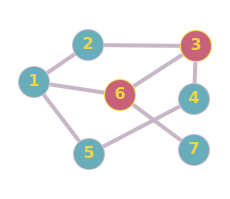
\includegraphics[width=0.3\textwidth]{figures7/vecindario.png}
        \caption{Para $S = \{3,6\}$ se tiene que $N(S) = \{1,2,3,4,6,7\}$}
    \end{subfigure} 
    \begin{subfigure}[b]{0.70\textwidth}
        \centering
        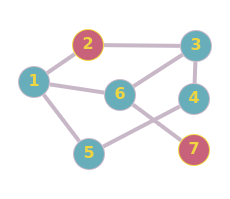
\includegraphics[width=0.3\textwidth]{figures7/vecindario2.png}
        \caption{Para $S = \{2,7\}$ se tiene que $N(S) = \{1,3,6\}$}
    \end{subfigure}
\end{figure} 

\begin{teo}
 \textbf{Teorema de Hall} Sea $G=<X\cup Y, E>$ un grafo bipartito con conjuntos X,Y entonces existe un emparejamiento que satura a X (emparejamiento completo) si y solo si para todo $S\subseteq X$ se cumple que $|N(S)|\geq |S|$
\end{teo}

\begin{dem}[$\Rightarrow$]
 
\end{dem}

Tomemos S, un subconjunto cualquiera de X, como en G hay un emparejamiento que satura a X, entonces al menos para cada vértice v de S existe un vértice w en Y tal que $\{v,w\}$ pertenece al emparejamiento y por tanto a N(S), luego N(S) tendrá al menos la misma cantidad de vértices que S, por tanto $|N(S)|\geq |S|$\\


\begin{dem}[$\Leftarrow$]
 
\end{dem}

Supongamos que $|N(S)|\geq |S|$ y que M es un emparejamiento máximo de G. Ahora, supongamos que existe un vértice $u\in X$ que no está saturado por M, entonces definimos un conjunto A formado por los vértices de G que pueden ser conectados con u a través de un camino M-alternativo. Se tiene $S=A\cap X$ y $T=A\cap Y$. Como M es máximo no hay caminos M-incremento. 

Por otra parte, por definición de T, todos los vértices de T pueden ser conectados con u por caminos alternados que empiezan por tanto con una arista que no pertenece a M (puesto que u no está saturado por M). Entonces todos los vértices de T han de estar emparejados por M con un vértice de $S- \{u\}$ (ya que de lo contrario, el camino alternado que les uniría con u sería un camino M-incremento, el cual no puede existir).

De igual manera, por definición de S, todos los vértices de S distintos de u pueden ser conectados con u a través de un camino alternado.  Como $u\in S$ pero no está saturado por M, para que dichos caminos sean alternados, deben llegar a los vértices de S por aristas pertenecientes a M.

De aquí deducimos que todo vértice de S, a excepción de u, está emparejado por M con un vértice de T. Por tanto, por definición de los conjuntos A, S y T, se llega a establecer una biyección entre el conjunto T y $S-\{ u \}$, luego $|T| = |S| - 1$ (puesto que $u \in S$).

Veamos ahora que $N(S)\subseteq  T$.

Sea $b\in N(S)$, entonces existe $a\in S$ tal que $\{a,b\}\in E(G)$. 
Como $a\in S$ existe un camino alternado que une a con u. Sea $c\in T$ tal que la última arista de dicho camino es $\{a,c\}\in M$ (esto porque no hay camino M-incremento), pueden darse dos situaciones:
\begin{itemize}
 \item Si $b=c$ entonces $\{a,b\}\in M$ y  $b\in T$
 \item Si $b\neq c$ entonces $\{a,b\}\not \in M$~(ya que a está emparejado con c por M) y por tanto $b\in T$ porque podría ser conectado con u a través del camino alternado que
une a con u añadiéndole la arista $\{a,b\}\not \in M$
\end{itemize}

Entonces tenemos que $|N(S)| \leq |T| = |S| - 1 < |S|$, lo cual es una contradicción con
nuestra hipótesis de partida ($|N(S)| \geq |S|$). Por tanto, concluimos que ese vértice $u$ no
saturado por M no puede existir $\blacksquare$.


\begin{cor}
 Sea $G=<X\cup Y, E>$ un grafo bipartito con conjuntos X,Y, $|X|\leq|Y|$. Si existe un número natural k tal que para todo $x\in X$ y para todo $y\in Y$, $deg(x)\geq k$ y $deg(y)\leq k$ entonces en G existe un emparejamiento que satura a X.
\end{cor}

\newpage

\begin{dem}
 
\end{dem}


Sea A un subconjunto de X. Como por hipítesis $deg(x)\geq k$ para todo vértice
$x \in X$, y $A \subseteq X$, entonces hay al menos $k|A|$ aristas con un extremo en A. 
El otro extremo de estas aristas está en N(A). 

Como, además, por hipótesis $deg(y) \leq k$ para todo $y \in Y $,
entonces también se cumple que todo $y \in N(A)$ es incidente en como mucho k aristas (ya
que al ser G bipartito $N(A) \subseteq Y$ ). Se puede ver que el número de vértices de N(A) es al menos $\frac{k|A|}{k} = |A|$. Aplicando entonces el Teorema de Hall, G tiene un emparejamiento completo de X en Y $\blacksquare$.

\begin{cor}
 Sea $G=<X\cup Y, E>$ un grafo bipartito regular de grado $r\geq 1$  entonces G
tiene un emparejamiento perfecto.
\end{cor}


\begin{dem}
 
\end{dem}


Si G es bipartito y regular con $r\geq 1$, entonces $r|X| = r|Y|$ y por tanto $|X|=|Y|$.
Sea $S \subseteq X$ un subconjunto no vacío cualquiera de X. Sea $E_1$ el conjunto de las
las aristas incidentes en S y $E_2$ el conjunto de las aristas incidentes en N(S). Por definición de N(S) tenemos que $E_1\subseteq E_2$. Entonces, si $|E_1|=r|S|$ y 
$|E_2|=r|N(S)|$ tenemos que $r|N(S)|\geq r|S|$ por lo que $|N(S)|\geq |S|$ $\blacksquare$.



\end{document} 
